\section{Pengantar Kriptografi Modern}
\label{sec:kriptografi-modern}

Kriptografi modern lahir bersama komputer digital pada awal dekade 1970-an.
Perubahan yang dibawanya bukan sekadar pergantian alat --- dari pena dan kertas
ke rangkaian elektronik --- melainkan pergantian \emph{satuan kerja}. Cipher
klasik pada Bab~\ref{chap:kriptografi-klasik} bekerja pada huruf: satu langkah
enkripsi memproses satu huruf, atau satu pasangan huruf. Algoritma modern
bekerja pada \textbf{bit} dan \textbf{byte}: plainteks, kunci, dan cipherteks
dipandang sebagai rangkaian bit, dan operasi dasarnya adalah operasi atas bit.
Konsekuensinya besar. Sebuah huruf yang sama dapat berubah menjadi cipherteks
yang berbeda pada setiap kemunculannya, dan ukuran kunci --- dinyatakan dalam
bit, bukan dalam jumlah huruf --- dapat dibuat sangat besar sehingga pencarian
menyeluruh menjadi mustahil.

Meski begitu, kriptografi modern tidak membuang warisan klasik. Dua teknik dasar
dari bab sebelumnya, \textbf{substitusi} dan \textbf{transposisi (permutasi)},
tetap menjadi kerangka algoritmanya; yang berubah adalah tingkat kerumitannya.
Substitusi tidak lagi berupa pergeseran tetap, melainkan tabel substitusi
(\textit{S-box}) yang dibangkitkan dengan aturan non-linier; transposisi tidak
lagi berupa pengacakan kolom, melainkan permutasi bit yang dikendalikan kunci.
Selain itu muncul teknik tambahan seperti rotasi, ekspansi, kompresi, dan
penjumlahan modulo $2^n$. Tujuannya satu: agar cipherteks tidak memperlihatkan
pola apa pun yang dapat dimanfaatkan kriptanalis.

Kriptografi modern juga melahirkan konsep-konsep yang tidak dikenal pada era
klasik: algoritma kunci-publik, fungsi \textit{hash}, protokol kriptografi,
tanda tangan digital, pembangkit bilangan acak, dan skema pembagian kunci.
Semua itu tersusun dalam sebuah hierarki yang menghubungkan kebutuhan keamanan
di tingkat tertinggi dengan primitif di tingkat terendah, sebagaimana
diperlihatkan pada Gambar~\ref{fig:kriptografi-modern-blok}.

\begin{figure}[htbp]
    \centering
    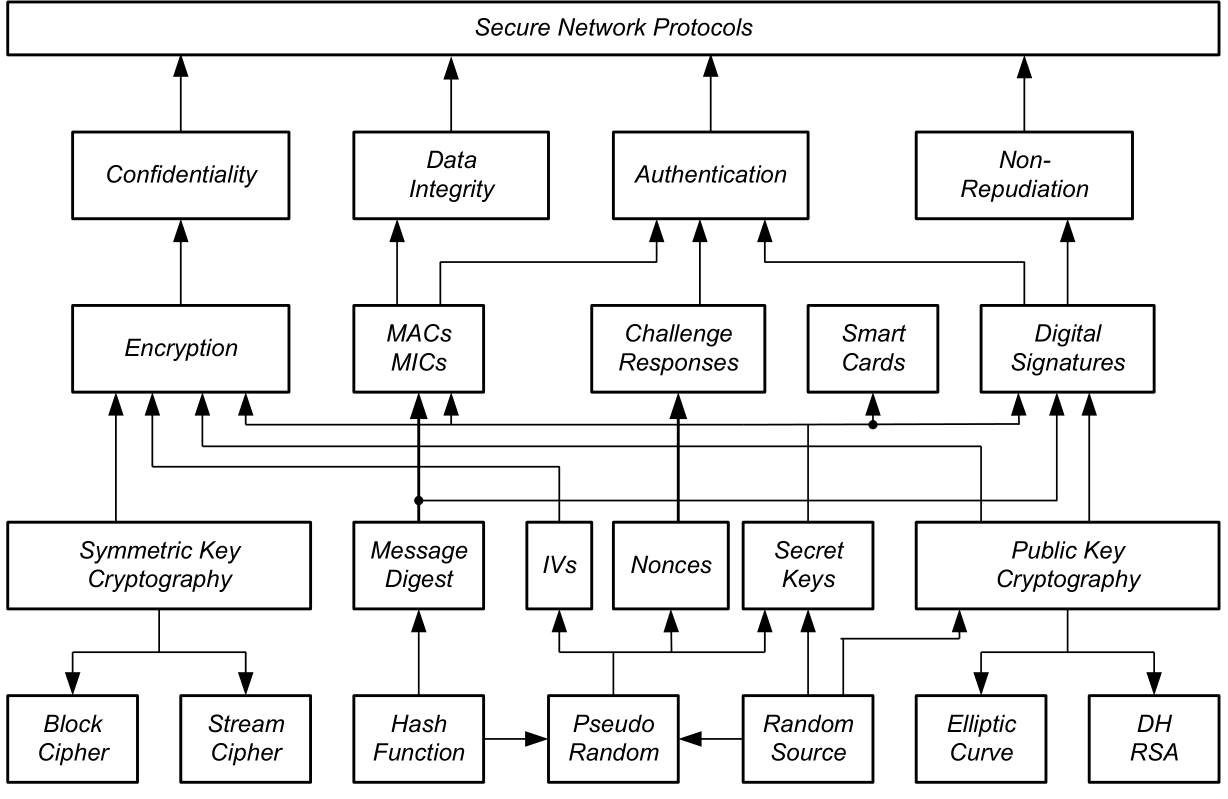
\includegraphics[width=0.72\linewidth, height=0.42\textheight, keepaspectratio]{figures/kriptografi-modern-blok.png}
    \caption{Diagram blok kriptografi modern: dari protokol jaringan aman di tingkat teratas turun ke tujuan
    keamanan, mekanisme, metode, dan akhirnya primitif kriptografi}
    \label{fig:kriptografi-modern-blok}
    \sumber{Munir, \textit{IF4020 Kriptografi}, ITB.}
\end{figure}

Hierarki itu dibaca dari atas ke bawah. Kebutuhan berkomunikasi secara aman
menuntut sejumlah \emph{tujuan keamanan} --- kerahasiaan, keutuhan data,
otentikasi, dan nir-penyangkalan --- yang telah dibahas pada
Bab~\ref{chap:layanan-keamanan}. Tujuan itu dicapai melalui \emph{mekanisme}:
enkripsi, kode otentikasi pesan (\textit{MAC}), tantangan--jawaban, dan tanda
tangan digital. Setiap mekanisme dibangun di atas \emph{metode} kriptografi ---
kunci simetris, \textit{message digest}, dan kunci publik --- yang pada akhirnya
bersandar pada \emph{primitif}: \textit{block cipher}, \textit{stream cipher},
fungsi \textit{hash}, pembangkit bilangan acak, dan operasi matematis seperti
kurva eliptik serta RSA. Bab ini berada pada tingkat primitif paling bawah,
yaitu \textbf{\textit{stream cipher}}, primitif simetris yang bekerja langsung
pada aliran bit.

\subsection{Karakteristik Utama}

Perubahan paradigma dari kriptografi klasik ke kriptografi modern dapat
diringkas menjadi tiga poin:

\begin{enumerate}
    \item \textbf{Representasi biner.} Data --- plainteks, kunci, dan cipherteks
          --- direpresentasikan sebagai rangkaian bit $0$ dan $1$. Tidak ada
          lagi pemetaan tetap dari huruf ke bilangan seperti pada Affine cipher;
          yang ada adalah rangkaian bit dengan panjang tertentu, misalnya plainteks
          sepanjang $n$ bit dan kunci sepanjang $k$ bit.
    \item \textbf{Operasi dasar.} Operasi \textbf{XOR} ($\oplus$) menjadi
          operasi yang paling dominan karena sangat efisien di perangkat keras
          maupun perangkat lunak, dan karena sifatnya yang membalik dirinya
          sendiri. Di samping XOR, algoritma modern memakai rotasi bit,
          penjumlahan modulo $2^{32}$, serta substitusi melalui \textit{S-box}.
    \item \textbf{Kompleksitas.} Meskipun tetap bertumpu pada substitusi dan
          transposisi, operasi modern diulang dalam banyak putaran
          (\textit{round}) dengan fungsi non-linier di antara putaran-putaran
          itu. Inilah yang membuat hubungan antara kunci dan cipherteks menjadi
          sangat rumit, sehingga serangan analitis menjadi jauh lebih mahal
          daripada pencarian kunci secara menyeluruh.
\end{enumerate}

Ringkasan perbedaan kedua era disajikan pada Tabel~\ref{tab:klasik-vs-modern}.

\begin{table}[htbp]
    \centering
    \caption{Perbandingan kriptografi klasik dan kriptografi modern}
    \label{tab:klasik-vs-modern}
    \begin{tabularx}{\linewidth}{|>{\raggedright\arraybackslash}p{3.0cm}|>{\raggedright\arraybackslash}X|>{\raggedright\arraybackslash}X|}
    \hline
    \textbf{Aspek} & \textbf{Kriptografi Klasik} & \textbf{Kriptografi Modern} \\
    \hline
    Unit pemrosesan & Karakter atau huruf & Bit, byte, atau blok bit \\
    \hline
    Operasi dominan & Substitusi dan transposisi manual & XOR, rotasi, penjumlahan modulo, dan fungsi non-linier \\
    \hline
    Ukuran kunci & Kecil, sering berupa kata kunci & Besar, puluhan hingga ratusan bit \\
    \hline
    Sumber keamanan & Kerahasiaan algoritma & Kerahasiaan kunci (Prinsip Kerckhoffs) \\
    \hline
    Media penerapan & Pena dan kertas & Perangkat keras dan perangkat lunak \\
    \hline
    Contoh algoritma & Caesar, Vigen\`ere, Playfair, Hill & DES, AES, RC4, ChaCha20 \\
    \hline
    Ketahanan terhadap pencarian menyeluruh & Lemah; ruang kunci ribuan hingga miliaran & Kuat bila kunci $\ge 128$ bit \\
    \hline
    \end{tabularx}
\end{table}

\subsection{Bit, Byte, dan Kode Heksadesimal}

Pesan di dalam cipher modern diproses bit demi bit, byte demi byte, atau dalam
kelompok bit yang lebih besar. Satuan dasarnya adalah byte, dan satu byte
terdiri atas delapan bit:
\[
1 \text{ byte} = 8 \text{ bit}.
\]
Karena rangkaian delapan bit sulit dibaca mata, penulisan sering dipadatkan ke
kode heksadesimal (\textbf{Hex}). Satu digit heksadesimal mewakili tepat empat
bit, sehingga dua digit heksadesimal setara dengan satu byte:
\[
1 \text{ digit hex} = 4 \text{ bit}.
\]
Contohnya, rangkaian 16 bit $1001110101101010$ dibagi menjadi empat kelompok
empat bit dan setiap kelompok diganti dengan digit heksadesimalnya:
\[
1001\ 1101\ 0110\ 1010 = \code{9D6A}.
\]
Tabel~\ref{tab:konversi-biner-hex} memuat konversi lengkap keempat bit menjadi
satu digit heksadesimal.

\begin{table}[htbp]
\centering
\small
\begin{tabular}{@{}c c @{\hspace{14pt}} c c @{\hspace{14pt}} c c @{\hspace{14pt}} c c@{}}
\hline
Biner & Hex & Biner & Hex & Biner & Hex & Biner & Hex \\
\hline
0000 & 0 & 0100 & 4 & 1000 & 8 & 1100 & C \\
0001 & 1 & 0101 & 5 & 1001 & 9 & 1101 & D \\
0010 & 2 & 0110 & 6 & 1010 & A & 1110 & E \\
0011 & 3 & 0111 & 7 & 1011 & B & 1111 & F \\
\hline
\end{tabular}
\caption{Konversi empat bit biner ke satu digit heksadesimal}
\label{tab:konversi-biner-hex}
\sumber{Data dari Munir, \textit{IF4020 Kriptografi}, ITB; tabel disusun dari tabel konversi tersebut.}
\end{table}

Hal yang sama berlaku untuk teks. Setiap karakter dikodekan menurut suatu tabel
kode karakter, umumnya ASCII untuk huruf Latin, sehingga kata \code{Halo}
menjadi rangkaian 32 bit:
\begin{center}
\texttt{01001000 01100001 01101100 01101111}.
\end{center}
Kalimat yang lebih panjang menghasilkan rangkaian yang jauh lebih panjang,
misalnya \code{Indonesia emas 2045} yang menempati 152 bit. Panjang inilah yang
menentukan ukuran kunci yang dibutuhkan: kunci delapan karakter sama dengan
kunci 64 bit, sedangkan kunci 32 karakter sama dengan 256 bit. Di dalam buku
ini, plainteks dan cipherteks dituliskan dalam biner ketika operasinya
ditunjukkan langkah demi langkah, dan dalam heksadesimal ketika hanya nilainya
yang perlu disebutkan.

\subsection{Operasi XOR dan Bitwise}

Operasi XOR (\textit{Exclusive OR}) adalah fondasi dari hampir semua cipher
modern. Tabel kebenarannya ditunjukkan pada Tabel~\ref{tab:kebenaran-xor}:
keluarannya bernilai $1$ hanya jika kedua operand berbeda.

\begin{table}[htbp]
    \centering
    \caption{Tabel kebenaran operasi XOR}
    \label{tab:kebenaran-xor}
    \begin{tabular}{|c|c|c|}
    \hline
    $a$ & $b$ & $a \oplus b$ \\
    \hline
    0 & 0 & 0 \\
    0 & 1 & 1 \\
    1 & 0 & 1 \\
    1 & 1 & 0 \\
    \hline
    \end{tabular}
\end{table}

XOR memiliki empat sifat yang dipakai berulang kali di dalam algoritma
kriptografi:

\begin{enumerate}
    \item $a \oplus a = 0$ --- sebuah nilai yang di-XOR dengan dirinya sendiri
          habis menjadi nol.
    \item $a \oplus 0 = a$ --- nol adalah unsur identitas.
    \item $a \oplus b = b \oplus a$ (komutatif).
    \item $a \oplus (b \oplus c) = (a \oplus b) \oplus c$ (asosiatif).
\end{enumerate}

Keempat sifat itu dapat diperiksa langsung dari tabel kebenaran: untuk setiap
pasangan nilai $a$ dan $b$ yang mungkin, kedua ruas selalu menghasilkan bit yang
sama. Yang paling penting bagi kriptografi adalah sifat pertama. Dengan sifat
itu, enkripsi dan dekripsi dapat memakai fungsi yang sama persis. Misalkan
cipherteks dihitung sebagai $c = p \oplus k$ yang dinyatakan pada
Persamaan~\ref{eq:xor-enkripsi}; penerima yang memiliki kunci $k$ yang sama
tinggal mengulang operasi yang sama, sebagaimana ditunjukkan pada
Persamaan~\ref{eq:xor-dekripsi}:

\begin{equation}
c = p \oplus k
\label{eq:xor-enkripsi}
\end{equation}

\begin{equation}
p' = c \oplus k = (p \oplus k) \oplus k = p \oplus (k \oplus k) = p \oplus 0 = p.
\label{eq:xor-dekripsi}
\end{equation}

Operasi ini diterapkan bit demi bit pada posisi yang bersesuaian, sehingga
sering disebut \textbf{\textit{bitwise XOR}}. Misalnya $10011 \oplus 11001$,
dihitung dari bit paling kanan ke paling kiri, menghasilkan $01010$ seperti
diperlihatkan pada Gambar~\ref{fig:xor-bitwise}.

\begin{figure}[htbp]
    \centering
    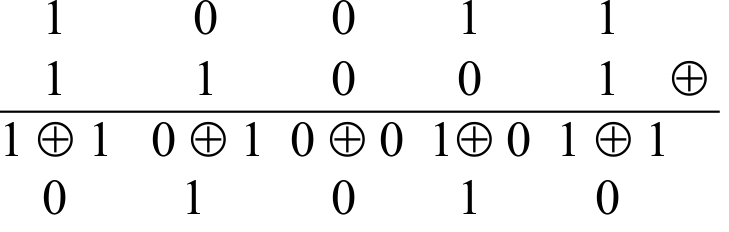
\includegraphics[width=0.45\linewidth, height=0.3\textheight, keepaspectratio]{figures/xor-bitwise.png}
    \caption{Perhitungan \textit{bitwise XOR} antara dua rangkaian bit dilakukan pada setiap posisi yang bersesuaian}
    \label{fig:xor-bitwise}
    \sumber{Munir, \textit{IF4020 Kriptografi}, ITB.}
\end{figure}

Pada data berukuran byte, hasil operasinya pun dapat dituliskan dalam
heksadesimal maupun sebagai karakter ASCII. Sebagai contoh, karakter \code{e}
bernilai $\code{65}$ dalam heksadesimal dan karakter \code{5} bernilai
$\code{35}$; hasil XOR keduanya adalah
\[
\code{65}_{16} \oplus \code{35}_{16} = \code{50}_{16},
\]
yaitu karakter \code{P}. Pasangan yang sama di-XOR sekali lagi mengembalikan
\code{e} tanpa perlu operasi khusus untuk dekripsi.

\subsection{Cipher XOR Sederhana dan Kelemahannya}

Bentuk paling sederhana dari cipher modern adalah \emph{Vigen\`ere cipher dalam
mode bit}: setiap bit plainteks di-XOR-kan dengan bit kunci, dan bila kunci
lebih pendek daripada pesan maka bit-bit kunci diulang secara periodik. Karena
aturan itu, cipher XOR sederhana mewarisi kelemahan cipher abjad-majemuk pada
Bab~\ref{chap:kriptografi-klasik}: periodisitas kunci dapat dilacak. Sebagai
ilustrasi, misalkan plainteks 29 bit dengan pola kunci yang berulang setiap tiga
bit:

\begin{center}
\small
\begin{tabular}{@{}ll@{}}
Plainteks  & \texttt{10010010101110101010001110001} \\
Kunci      & \texttt{11011011011011011011011011011} \\
Cipherteks & \texttt{01001001110101110001010101010} \\
\end{tabular}
\end{center}

\noindent
Kelemahan pertama tampak dari pola kunci itu. Kunci sepanjang 29 bit tersebut
hanyalah pengulangan pola tiga bit \code{110}, sehingga bit plainteks pada posisi
$i$, $i+3$, $i+6$, dan seterusnya semuanya di-XOR dengan bit kunci yang sama.
Semakin pendek periodenya, semakin banyak bit plainteks yang berbagi bit kunci:
pola tiga bit berarti hanya tiga bit kunci yang perlu ditebak, dan bit-bit
plainteks pada setiap kelas posisi dapat dipisahkan lalu digempur dengan analisis
frekuensi. Kriptanalis dapat menemukan panjang periode itu dengan cara yang sama
seperti metode Kasiski: menggeser cipherteks terhadap dirinya sendiri dan mencari
pergeseran yang membuat banyak bit bersesuaian, yang menandakan bahwa
posisi-posisi itu memakai ulang bit kunci yang sama.

Kelemahan kedua muncul ketika kunci yang sama dipakai untuk dua pesan berbeda.
Misalkan $c_1 = p_1 \oplus k$ dan $c_2 = p_2 \oplus k$. Bila kedua cipherteks itu
di-XOR-kan, kunci $k$ saling menghapus dan yang tersisa adalah XOR kedua
plainteksnya:
\[
c_1 \oplus c_2 = (p_1 \oplus k) \oplus (p_2 \oplus k) = p_1 \oplus p_2.
\]
Penyerang tidak perlu mengetahui kuncinya untuk memperoleh hubungan langsung
antara dua plainteks. Bila salah satu plainteks dapat diduga --- misalnya karena
format berkasnya dikenal, atau karena potongan teksnya berulang --- maka
plainteks yang lain dapat dipulihkan huruf demi huruf. Kelemahan ini muncul
berulang kali pada Bab~\ref{chap:kriptografi-klasik} sebagai serangan
\textit{two-time pad} terhadap One-Time Pad.

Dua kelemahan di atas menjelaskan mengapa cipher XOR sederhana tidak dipakai
apa adanya. Yang dibutuhkan bukan sekadar operasi XOR, melainkan
\textbf{keystream generator} yang membangkitkan aliran bit kunci yang panjangnya
sama dengan pesan, dan yang mengubah kunci pendek menjadi keystream tanpa pola
yang dapat dilacak. Keystream generator itulah yang menjadi pokok bahasan
Bagian~\ref{sec:konsep-stream-cipher}.
